\documentclass[10pt, aspectratio=169]{beamer}
% \documentclass[11pt,handout]{beamer}
\usepackage[T1]{fontenc}
\usepackage[utf8]{inputenc}
\usepackage{textcomp}
\usepackage{float, afterpage, rotating, graphicx}
\usepackage{epstopdf}
\usepackage{longtable, booktabs, tabularx}
\usepackage{fancyvrb, moreverb, relsize}
\usepackage{eurosym, calc}
\usepackage{amsmath, amssymb, amsfonts, amsthm, bm}
\usepackage[
    natbib=true,
    bibencoding=inputenc,
    bibstyle=authoryear-ibid,
    citestyle=authoryear-comp,
    maxcitenames=3,
    maxbibnames=10,
    useprefix=false,
    sortcites=true,
    backend=biber
]{biblatex}

% for figures
\usepackage{subcaption}
\usepackage[english]{babel}

\usepackage{graphicx}
\graphicspath{{../bld/python/figures/}}

% for csv tables
\usepackage{siunitx,array,booktabs}
\usepackage{csvsimple}
\usepackage{adjustbox}

\AtBeginDocument{\toggletrue{blx@useprefix}}
\AtBeginBibliography{\togglefalse{blx@useprefix}}
\setlength{\bibitemsep}{1.5ex}
\addbibresource{references.bib}
\usepackage{biblatex}

\hypersetup{colorlinks=true, linkcolor=black, anchorcolor=black, citecolor=black, filecolor=black, menucolor=black, runcolor=black, urlcolor=black}

\setbeamertemplate{footline}[frame number]
\setbeamertemplate{navigation symbols}{}
\setbeamertemplate{frametitle}{\centering\vspace{1ex}\insertframetitle\par}
\setbeamertemplate{caption}[numbered]

\begin{document}

\title{Crime Data Mapping and Spatial Regression}

\author[Mudabbira Mushtary]
{
{\bf Mudabbira Mushtary}\\
{\small University of Bonn}\\[1ex]
}


\begin{frame}
    \titlepage
    \note{~}
\end{frame}

%% Slide with a figure and text in two seperate columns
\begin{frame}{Point Patterns of Burglary Incidents}
    \begin{columns}
        % Column 1
        \begin{column}{0.5\textwidth}
            \begin{itemize}
                \item \textbf{Kernel density estimates:} Counting the number of points in a continuous way.
                \item Burglaries are centered around the city center.
            \end{itemize}
        \end{column}
        % Column 2
        \begin{column}{0.5\textwidth}
            \begin{figure}
            \centering
                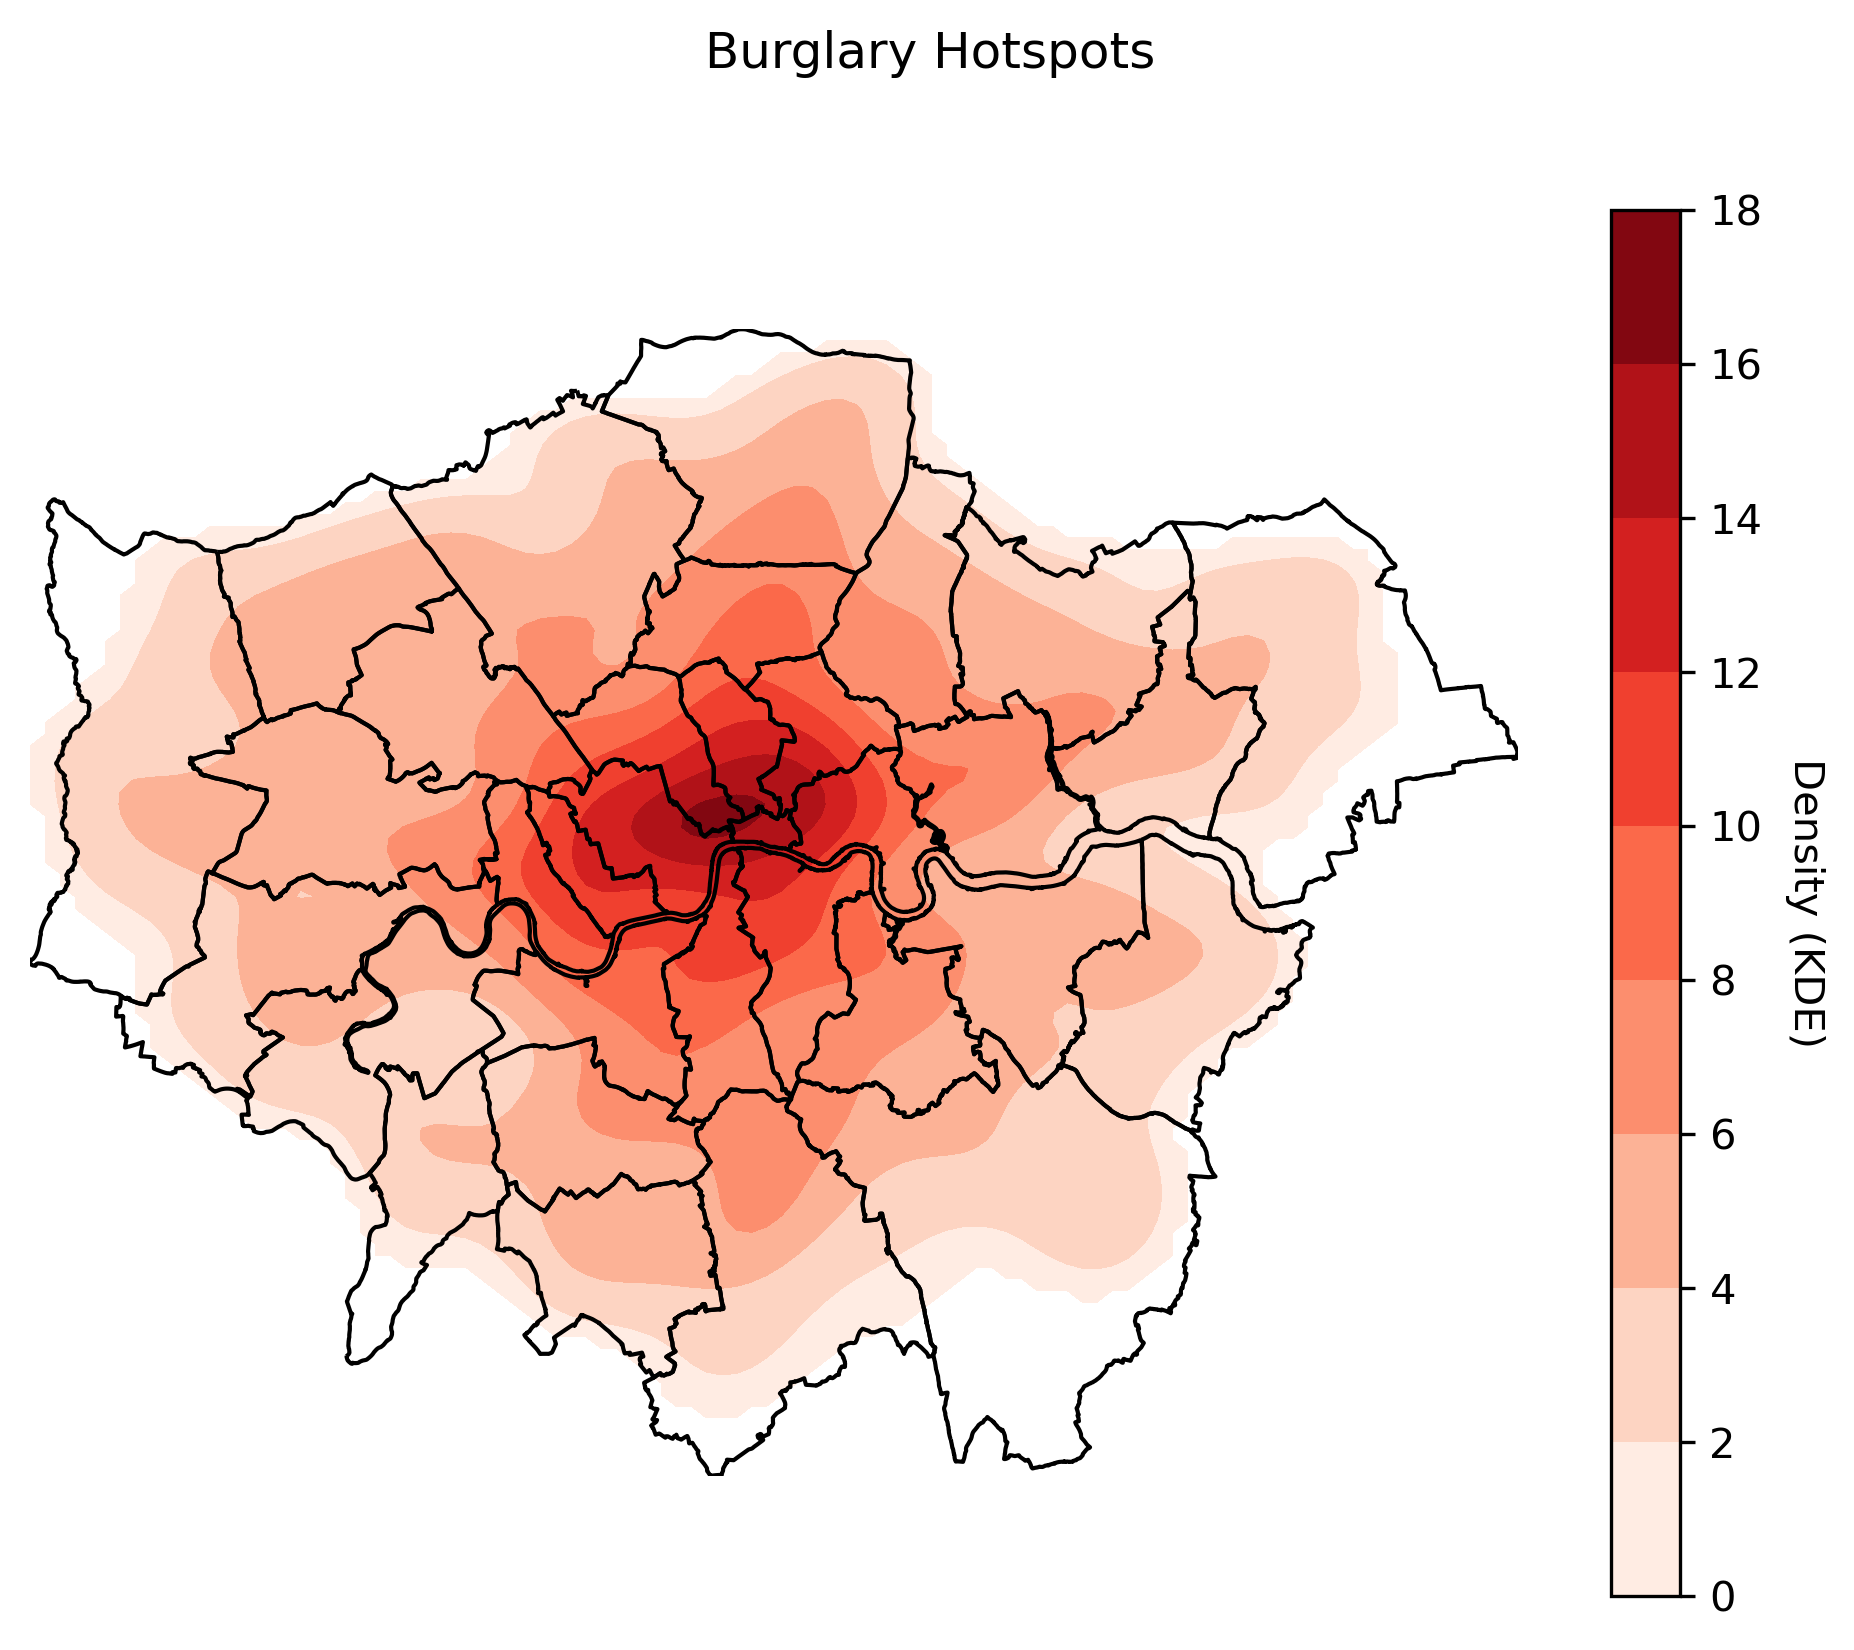
\includegraphics[width=1.0\textwidth]{burglary_hotspots.png}
                \caption{Burglary hotspots within greater London Area.}
            \end{figure}
        \end{column}
    \end{columns}
\end{frame}

%% Slide with a figure and text in two seperate columns
\begin{frame}{Spatial Clustering of Burglary Incidents}
    \begin{columns}
        % Column 1
        \begin{column}{0.5\textwidth}
            \begin{itemize}
                \item \textbf{DBSCAN:} density-based clustering
                \item \textbf{Assumption}: clusters are dense regions in space separated by regions of lower density
                \item Burglaries are centered around the city center.
            \end{itemize}
        \end{column}
        % Column 2
        \begin{column}{0.5\textwidth}
            \begin{figure}
            \centering
                \includegraphics[width=1.0\textwidth]{burglary_clusters.png}
                \caption{Burglary clusters within greater London Area.}
            \end{figure}
        \end{column}
    \end{columns}
\end{frame}

%% Slide with a figure and text in two seperate columns
\begin{frame}{Spatial Weights Matrix}
    \begin{columns}
        % Column 1
        \begin{column}{0.5\textwidth}
            \begin{itemize}
                \item A spatial weights matrix is the way geographical space is formally encoded into
                a numerical form so it is easy for a computer (or a statistical method) to understand.
                \item We can define a spatial weights matrix, such as contiguity, distance-based,
                or block. The following analysis has used a Queen contiguity matrix.
                \item \textbf{Queen Contiguity Matrix:} For a pair of local authorities in the dataset to be
                considered neighbours under this W, they will need to be sharing border or, in other words, “touching” each other to some degree.

            \end{itemize}
        \end{column}
        % Column 2
        \begin{column}{0.5\textwidth}
            \begin{figure}
            \centering
                \includegraphics[width=1.0\textwidth]{weights_matrix_ward.png}
                \caption{Burglary clusters within greater London Area.}
            \end{figure}
        \end{column}
    \end{columns}
\end{frame}

%% Slide with two figures and text
\begin{frame}{Spatial Lag of Burglary Incidents}
    \textbf{Spatial lag} is a spatially weighted average of the values of a
    variable in the neighbourhood of each observation.Once we have weights matrix,
    we can look at the spatial lag of the burglary in the Greater London area

    %You can see in Figure \ref{fig:images} that I have inserted two images, Figures \ref{fig:nature1} and \ref{fig:nature2}, that I can reference independently. More text, More text, More text, More text, More text,More text ,More text
    \begin{figure}
        \centering
            \begin{subfigure}[t]{0.4\textwidth}
                \includegraphics[width=\textwidth]{burglary_ward.png}
                \caption{No. of Burglary Incidents (2019)}\label{fig:burglary}
            \end{subfigure}
            \begin{subfigure}[t]{0.4\textwidth}
                \includegraphics[width=\textwidth]{burglary_ward_lag.png}
                \caption{Burglary Lag (2019)}\label{fig:burglary_lag}
            \end{subfigure}
        \caption{Burglary incidents and the corresponding lag on a ward level.}\label{fig:lag}
    \end{figure}
\end{frame}



%% Slide with two figures and text
\begin{frame}{Moran Plot}
    \begin{itemize}
        \item \textbf{} The plot displays a positive relationship between the standardized rate of burglary and its spatial lag.
     
    \end{itemize}
    
    %You can see in Figure \ref{fig:images} that I have inserted two images, Figures \ref{fig:nature1} and \ref{fig:nature2}, that I can reference independently. More text, More text, More text, More text, More text,More text ,More text
    \begin{figure}
        \centering
            \begin{subfigure}[t]{0.4\textwidth}
                \includegraphics[width=\textwidth]{moran_scatter.png}
                \caption{Moran's Plot}\label{fig:moran_scatter}
            \end{subfigure}
            \begin{subfigure}[t]{0.4\textwidth}
                \includegraphics[width=\textwidth]{moran_distribution.png}
                \caption{Distribution after random Sampling}\label{fig:moran_distribution}
            \end{subfigure}
        \caption{Moran's I and Global Spatial Autocorrelation}\label{fig:moran}
    \end{figure}
\end{frame}

\begin{frame}{Moran Plot}
    \begin{itemize}
        \item Moran plot is a way of visualizing a spatial dataset to explore the nature and strength of spatial autocorrelation.
        \item This is associated with the presence of \textbf{positive spatial autocorrelation:} similar values tend to be located close to each other. This means that the \textbf{overall trend} is for high values to be close to other high values, and for low values to be surrounded by other low values.
    \end{itemize}
    
\end{frame}


\begin{frame}{Moran's I and Spatial Autocorrelation}
    \begin{itemize}
        
        \item \textbf{Moran's I} is a measure of \textbf{spatial autocorrelation}.
        \item From the figure \ref{fig:moran_scatter}, we can see that the value of the Moran's I is 0.5, which is a positive value.
        \item With the small p-value associated with the Moran's I, we can conclude that the map displays 
        more spatial pattern that we would expect if the values had been randomly allocated to a particular location.
        \item \textbf{Global Spatial Autocorrelation} relates to the overall geographical pattern present in the data.
        \item Global autocorrelation analysis shows us that observations do seem positively correlated over space. 


    \end{itemize}
   
    %You can see in Figure \ref{fig:images} that I have inserted two images, Figures \ref{fig:nature1} and \ref{fig:nature2}, that I can reference independently. More text, More text, More text, More text, More text,More text ,More text
   
\end{frame}

%% Slide with two figures and text
\begin{frame}{Resource Deprivation in Greater London Area}
    Resource deprivation scores on a LSOA level as shown in Figure \ref{fig:imd_scores_lsoa}
    have been aggregated to a ward level for subsequent spatial regression analysis
    as shown in Figure \ref{fig:imd_scores_ward}.
    \begin{figure}
        \centering
            \begin{subfigure}[t]{0.4\textwidth}
                \includegraphics[width=\textwidth]{imd_scores_lsoa.png}
                \caption{Indices of Multiple Deprivation LSOA level}\label{fig:imd_scores_lsoa}
            \end{subfigure}
            \begin{subfigure}[t]{0.4\textwidth}
                \includegraphics[width=\textwidth]{imd_scores_ward.png}
                \caption{Indices of Multiple Deprivation on ward level}\label{fig:imd_scores_ward}
            \end{subfigure}
        \caption{English Indices of Multiple Deprivation (IMD)}\label{fig:imd}
    \end{figure}
\end{frame}


%% Slide with two figures and text
\begin{frame}{Spatial Regression: Burglaries and Resource Deprivation}
    Number of burglaries a shown in in Figure \ref{fig:burglary_ward} and resource deprivation as shown
    in Figure \ref{fig:imd_scores_ward} are used for spatial regression analysis on a ward level.
    \begin{figure}
        \centering
            \begin{subfigure}[t]{0.4\textwidth}
                \includegraphics[width=\textwidth]{burglary_ward.png}
                \caption{Indices of Multiple Deprivation LSOA level}\label{fig:burglary_ward}
            \end{subfigure}
            \begin{subfigure}[t]{0.4\textwidth}
                \includegraphics[width=\textwidth]{imd_scores_ward.png}
                \caption{Indices of Multiple Deprivation on ward level}\label{fig:imd_scores_ward}
            \end{subfigure}
        \caption{English Indices of Multiple Deprivation (IMD)}\label{fig:burg_imd}
    \end{figure}
\end{frame}

% Slide with table
\begin{frame}{Spatial Regression}
    
    \small\begin{table}[!h]
        \input{../bld/python/tables/model_spatial_ols_summary.tex}
        \caption{\label{tab:ols_summary} Estimation results of regression.}
    \end{table}
    \begin{itemize}
        \item \textbf{Independent variables:} Resource deprivation scores.
        \item \textbf{Dependent Variable:} Burglary rate in GreaterLondon Area .
        \item \textbf{Null hypothesis:} No Spatial autocorrelation in the residuals.
        \item \textbf{Alternative hypothesis:} There is spatial autocorrelation in the residuals. 
        \item \textbf{Conclusion:} The null hypothesis is rejected. There is spatial autocorrelation in the residuals.
    \end{itemize}
\end{frame}

% Slide with table
\begin{frame}{Spatial Regression}

    \begin{adjustbox}{max width=\textwidth, keepaspectratio, rotate=0, caption={Spatial Diagnostic Tests}, float=table}
        \input{../bld/python/tables/spat_diag_ols_tex.tex}
    \end{adjustbox}\label{tab:spat_diag}
    
    \begin{itemize}
        \item \textbf{Lagrange Multiplier Tests} suggests that a spatial error or spatial lag model would improve the fit of our model.
        \item We have got significant results for both LM error and LM lag. This shows that we should consider the spatial correlation. 
        \item However, according to the Robust LM and Robust LM(error) values, we should only consider the Spatial Error model as Robust LM is not significant anymore.
        \item We will continue with the spatial error and spatial lag models even though the error model is more than likely the correct path. 
    \end{itemize}
    
\end{frame}

\begin{frame}{Spatial Regression: ML\_Lag}
    \begin{equation} 
        y_i=X_i \beta+\lambda w_i \epsilon_i+u_i
    \end{equation}
    \begin{itemize}
         
        \item \textbf{Spatial Lag Model} is a global model where the dependent variable among where neighbors influence the dependent variable. 
        \item \textbf{}For Example, If burglary incidence is higher in the neighborhood of the City Centre of London, its highly likely to have high burglary incidence in the city center of London. Therefore, there is a feedback loop that occurs where affects on our neighbor(s) y affects our y and our neighbor(s) y variable.
        \item \textbf{Null hypothesis:} Spatial dependencies are not captured by the spatial lag Wy in the endogenous variable Y
        \item \textbf{Alternative hypothesis:} Spatial dependencies are captured by the spatial lag Wy in the endogenous variable Y
        
    \end{itemize}
\end{frame}

% Slide with table
\begin{frame}{Spatial Regression: ML\_Lag}
    \small\begin{table}[!h]
        \input{../bld/python/tables/model_spatial_ml_lag_summary.tex}
        \caption{\label{tab:ml_lag_summary} Estimation results of ML\_Lag regression.}
    \end{table}
    \begin{itemize}
         
        \item \textbf{W\_burglaryRate2019} is a spatially lagged y multiplier. 
        \item \textbf{} Coefficient is 0.84 (with a significant p-value)
        \item \textbf{} Burglary incidence tends to higher in an area when it is higher in the neighborhood with some spillover effects.  
        
    \end{itemize}
\end{frame}

\begin{frame}{Spatial Regression: ML\_Error}

    \begin{equation} 
        y_i=X_i \beta+\lambda w_i \epsilon_i+u_i
    \end{equation}
    
    \begin{itemize}
         
        \item \textbf{Spatial Error Model} does not include lagged dependent or independent variables, but instead includes a function of our unexplained error and that of our neighbors.
        \item \textbf{}Higher than expected residual values suggest a missing explanatory variable that is spatially correlated. In this analysis, Lambda is the error multiplier.
        \item \textbf{Null hypothesis:} There is no dependency of error values of an area with errors in other areas associated with it
        \item \textbf{Alternative hypothesis:} There is dependency of error values of an area with errors in other areas associated with it
        
    \end{itemize}
\end{frame}

% Slide with table
\begin{frame}{Spatial Regression: ML\_Error}
    \small\begin{table}[!h]
        \input{../bld/python/tables/model_spatial_ml_error_summary.tex}
        \caption{\label{tab:ml_error_summary} Estimation results of ML\_Error regression.}
    \end{table}
    \begin{itemize}
         
        \item \textbf{}Lambda coefficient is 0.86 with a significant p-value.
        \item \textbf{}Thus, we reject the null hypothesis and conclude that there is dependency of error values of an area with errors in other areas associated with it.
              
    \end{itemize}
    
\end{frame}

\begin{frame}{Model Compasiron and Conclusion}


    \small\begin{table}[!h]
        \input{../bld/python/tables/ml_lag_stats.tex}
        \caption{\label{tab:ml_lag_stats} Statistics of ML\_Lag model.}
    \end{table}

    \small\begin{table}[!h]
        \input{../bld/python/tables/ml_error_stats.tex}
        \caption{\label{tab:ml_error_stats} Statistics of ML\_Error model.}
    \end{table}
    
\end{frame}

\begin{frame}{Model Compasiron and Conclusion}

    \begin{itemize}
         
        \item \textbf{}We got lower log-likelihood for the Error model.In addition, Schwarz criterion of the error model is also lower than the lag model.
        \item \textbf{}So, we can conclude that this research is missing spatially correlated independent variable.
        \item \textbf{}Further work on this area is necessary to find the correct explanatory variables that are more appropriate for explaining burglary incidence in Greater London Area.
        
    \end{itemize}
    
\end{frame}


%% Slide with citation
\begin{frame}[t]
    \frametitle{Resources}
    Raw data was gathered from the following sources:
    \begin{itemize}
        \item Crime data is taken from \url{https://data.police.uk/data/}
        \item Deprivation data is taken from \url{https://www.gov.uk/government/statistics/english-indices-of-deprivation-2019}
    \end{itemize}

    Methods were selected from the following sources:
    \begin{itemize}
        \item Geospatial analysis: \citet{lawhead2019learning}
        \item Spatial Econometrics: \citet{anselin1988spatial} and \citet{kopczewska2020applied}
    \end{itemize}

    LaTeX template was taken from \citet{GaudeckerEconProjectTemplates} and modified.

    \note{~}
\end{frame}

\begin{frame}[allowframebreaks]
    \frametitle{References}
    \renewcommand{\bibfont}{\normalfont\footnotesize}
    \printbibliography
\end{frame}

\end{document}
